\setAuthor{Hans Daniel Kaimre}
\setRound{lõppvoor}
\setYear{2024}
\setNumber{G 1}
\setDifficulty{1}
\setTopic{TODO}

\prob{Kelgumägi}
\begin{wrapfigure}{r}{0.3\textwidth}
  \vspace*{-5mm}
    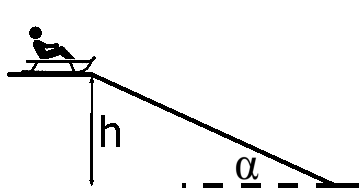
\includegraphics[width=0.3\textwidth]{2024-v3g-01-yl.pdf}
\end{wrapfigure}
Triinu ja Sandra on koos kelgutamas kelgumäel, mis on $h=\SI{6}{\m}$ kõrgune ning $\alpha=\SI{15}{\degree}$ ühtlase tõusunurgaga kogu nõlva ulatuses. Kui suure kiiruse peab Triinu Sandrale kelgumäe üleval sisse lükkama, et ta jõuaks mäest alla? Hõõrdetegur kelgu ning lumise nõlva vahel on $\mu=\num{0.3}$, raskuskiirendus $g=\SI{9.8}{\m\per\s\squared}$.


\hint

\solu
Lähendame Sandrat mäest alla kelgutades klotsina kaldpinnal (vt joonist). Sandrale mõjub raskusjõud $F_r=mg$, mille kaldpinna suunaline komponent on $mg\sin\alpha$ ning pinnanormaali suunaline komponent on $mg\cos\alpha$. Pinnanormaali suunaline komponent on võrdne toereaktsiooniga, st $N=mg\cos\alpha$. Kelgule mõjuv liughõõrdejõud on võrdeline toereaktsiooni ja jõõrdeteguriga: $F_h=\mu N=\mu mg\cos\alpha$. Seega Sandrat nõlval pidurdav jõud on $F_p = mg(\mu \cos\alpha - \sin\alpha)$, kust kiirendus $a=F_p/m=g(\mu \cos\alpha - \sin\alpha)$.
\begin{center}
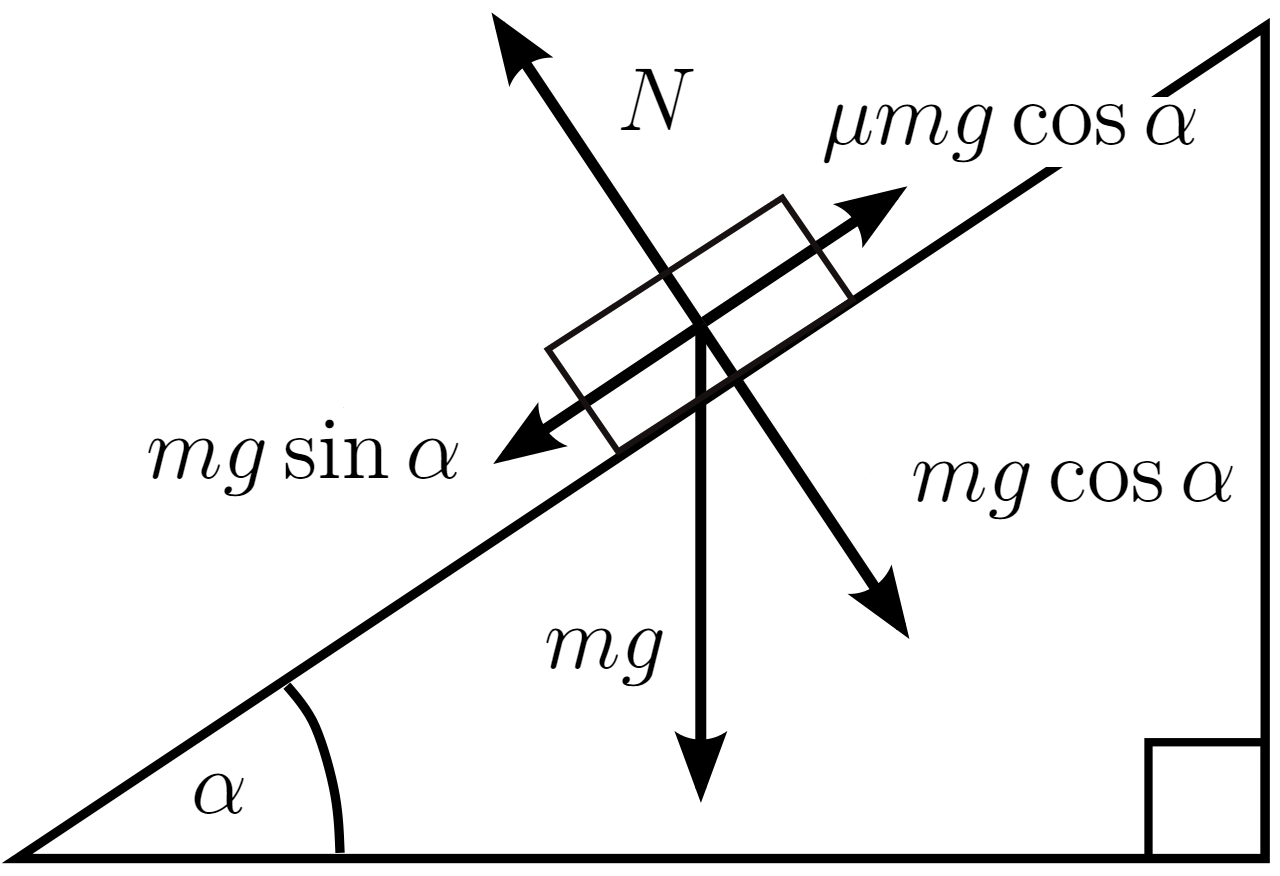
\includegraphics[width=0.45\textwidth]{2024-v3g-01-sol.png}
\end{center}
Ühtlase kiirendusega liikumise kirjeldamiseks kehtib valem $s=(v^2-v_0^2)/2a$, kus $s$ on nihe, $v$ keha lõppkiirus, $v_0$ keha algkiirus ning $a$ kehale mõjuv kiirendus. Piirjuhul jääb Sandra nõlva lõppu jõudes seisma, st $v=0$, kiirendus $a=-g(\mu \cos\alpha - \sin\alpha)$ (miinusmärgiga, kuna kiirendus on keha liikumise suunaga võrreldes vastassuunas) ning nihke leiame trigonomeetriast: $s=h/\sin\alpha$. Seega
\[
  \frac{h}{\sin\alpha} = \frac{-v_0^2}{-2g(\mu \cos\alpha - \sin\alpha)}.
\]
Millest
\begin{align*}
  v_0 &= \sqrt{\frac{2hg(\mu \cos\alpha - \sin\alpha)}{\sin\alpha}}\\
  &= \sqrt{\frac{2\cdot\SI{6}{\m}\cdot \SI{9.8}{\m\per\s\squared}  \cdot (0.3\cdot \cos \SI{15}{\degree}  - \sin\SI{15}{\degree})}{\sin\SI{15}{\degree}}} = \SI{3.8}{\m\per\s}.
\end{align*}
\probend